\section{Problema 5}

¿Cuántos números entre 300 y 900 son múltiplos de 2 o 5, pero no de 6?
\begin{solution}
El problema lo podemos visualizar como: 
\begin{center}
    

\tikzset{every picture/.style={line width=0.75pt}} %set default line width to 0.75pt        

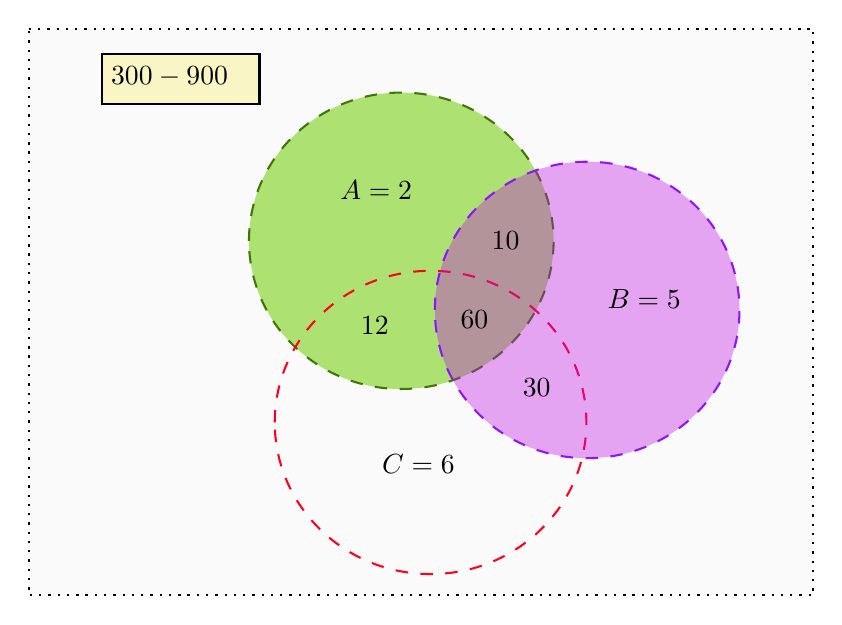
\begin{tikzpicture}[x=0.75pt,y=0.75pt,yscale=-1,xscale=1]
%uncomment if require: \path (0,300); %set diagram left start at 0, and has height of 300

%Shape: Rectangle [id:dp7203045602613047] 
\draw  [fill={rgb, 255:red, 0; green, 0; blue, 0 }  ,fill opacity=0.02 ][dash pattern={on 0.84pt off 2.51pt}] (125.43,17) -- (503.43,17) -- (503.43,290) -- (125.43,290) -- cycle ;
%Shape: Ellipse [id:dp05198513027857288] 
\draw  [color={rgb, 255:red, 65; green, 117; blue, 5 }  ,draw opacity=1 ][fill={rgb, 255:red, 126; green, 211; blue, 33 }  ,fill opacity=0.62 ][dash pattern={on 4.5pt off 4.5pt}] (231.55,119.17) .. controls (231.55,79.73) and (264.4,47.76) .. (304.93,47.76) .. controls (345.45,47.76) and (378.31,79.73) .. (378.31,119.17) .. controls (378.31,158.61) and (345.45,190.58) .. (304.93,190.58) .. controls (264.4,190.58) and (231.55,158.61) .. (231.55,119.17) -- cycle ;
%Shape: Ellipse [id:dp12947926731616155] 
\draw  [color={rgb, 255:red, 255; green, 0; blue, 31 }  ,draw opacity=1 ][fill={rgb, 255:red, 208; green, 2; blue, 27 }  ,fill opacity=0 ][dash pattern={on 4.5pt off 4.5pt}] (243.97,206.69) .. controls (243.97,166.34) and (277.58,133.63) .. (319.04,133.63) .. controls (360.5,133.63) and (394.11,166.34) .. (394.11,206.69) .. controls (394.11,247.04) and (360.5,279.75) .. (319.04,279.75) .. controls (277.58,279.75) and (243.97,247.04) .. (243.97,206.69) -- cycle ;
%Shape: Ellipse [id:dp04922743105309446] 
\draw  [color={rgb, 255:red, 144; green, 19; blue, 254 }  ,draw opacity=1 ][fill={rgb, 255:red, 189; green, 16; blue, 224 }  ,fill opacity=0.37 ][dash pattern={on 4.5pt off 4.5pt}] (321.11,152.49) .. controls (321.11,113.06) and (353.96,81.08) .. (394.49,81.08) .. controls (435.01,81.08) and (467.87,113.06) .. (467.87,152.49) .. controls (467.87,191.93) and (435.01,223.9) .. (394.49,223.9) .. controls (353.96,223.9) and (321.11,191.93) .. (321.11,152.49) -- cycle ;

% Text Node
\draw  [fill={rgb, 255:red, 248; green, 231; blue, 28 }  ,fill opacity=0.24 ]  (160.62,29.35) -- (236.62,29.35) -- (236.62,53.35) -- (160.62,53.35) -- cycle  ;
\draw (163.62,33.57) node [anchor=north west][inner sep=0.75pt]    {$300-900$};
% Text Node
\draw (274.08,88.68) node [anchor=north west][inner sep=0.75pt]    {$A=2$};
% Text Node
\draw (402.84,141.23) node [anchor=north west][inner sep=0.75pt]    {$B=5$};
% Text Node
\draw (294.25,220.69) node [anchor=north west][inner sep=0.75pt]    {$C=6$};
% Text Node
\draw (347,113.21) node [anchor=north west][inner sep=0.75pt]    {$10$};
% Text Node
\draw (284,154.21) node [anchor=north west][inner sep=0.75pt]    {$12$};
% Text Node
\draw (362,184.21) node [anchor=north west][inner sep=0.75pt]    {$30$};
% Text Node
\draw (332,151.21) node [anchor=north west][inner sep=0.75pt]    {$60$};


\end{tikzpicture}
\end{center}
Es decir, que nos interesa conocer los números del círculo verde y purpura; evitando \textbf{todos} los elementos del círculo punteado rojo. Ya que tenemos 3 conjuntos, vamos a usar la generalización del principio de inclusión-exclusión centrado para 3 conjuntos. Entonces,

$$\left|\bigcup_{i=1}^n A_i\right| = \sum_{i=1}^n |A_i| - \sum_{1 \leqslant i < j \leqslant n} |A_i\cap A_j| + \sum_{1 \leqslant i < j < k \leqslant n} |A_i \cap A_j\cap A_k| - \cdots + (-1)^{n-1} \left|A_1\cap\cdots\cap A_n\right|.$$
En el caso específico de n=3 (3 conjuntos), 

$$|A \cup B \cup C| = |A| + |B| + |C| - |A \cap B| - |A \cap C| - |B \cap C| + |A \cap B \cap C|.$$


\linita 

Elementos del conjunto $A$: 

$$A=\floor*{\frac{900}{2}}-\floor*{\frac{300}{2}}=300$$

Elementos del conjunto $B$: 

$$B=\floor*{\frac{900}{5}}-\floor*{\frac{300}{5}}=120$$

Elementos del conjunto $C$: 

$$C=\floor*{\frac{900}{6}}-\floor*{\frac{300}{6}}=100$$

\linita 

Elementos de $|A\cap B|$: 

$$A\cap B=\floor*{\frac{900}{2*5}}-\floor*{\frac{300}{2*5}}=60$$

Elementos de $|A\cap C|$: 
$$A\cap C=\floor*{\frac{900}{2*6}}-\floor*{\frac{300}{2*6}}=50$$
\newpage
Elementos de $|B\cap C|$: 

$$B\cap C=\floor*{\frac{900}{5*6}}-\floor*{\frac{300}{5*6}}=20$$

Elementos de $|A\cap B\cap C|$: 
$$A\cap B\cap C=\floor*{\frac{900}{2*5*6}}-\floor*{\frac{300}{2*5*6}}=10$$

\linita

Entonces, por el principio de inclusión-exclusión (excluyendo el conjunto $C$ porque no nos interesa), 
$$|A\cup B\cup C|= 300+120+0-60-50-20+10=300 \text{ números.}$$



\end{solution}